\documentclass[a4paper, 10pt, final]{article}
\usepackage{bonde}

\def\mytitle{Signal and Image Processing 2010}
\def\mysubtitle{Handin of mandatory excercise 2}
\def\myauthor{Ulrik Bonde}
\def\mymail{\mailto{bonde@diku.dk}}
\def\mydate{\today}

\title{\mytitle}
\subtitle{\mysubtitle}

\author{\myauthor{} - \mymail}
\date{\mydate}

\hypersetup{
colorlinks,%
citecolor=black,%
filecolor=black,%
linkcolor=black,%
urlcolor=black,%
bookmarksopen=false,
pdftitle={\mytitle{} - \mysubtitle},
pdfauthor={\myauthor}
}

\begin{document}
\maketitle

\subsection*{Question 2.1}
Listing \ref{fft_matlab} shows how MATLAB can be used to show the
Fourier transform of an image. I have found the Fourier transform for
two images shown in fig. \ref{fourier_transforms}.

The two original images are very different. The first shows only a white
box on a black background while the second shows some buildings. The
second image is blurred and noisy.

The Fourier transform of the first image is almost symmetric in the
white cross. The cross and the symmetry indicates some noticeable
periodic changes in both dimensions in the original image. Also, the
Fourier transformed image are segmented by black lines which further
indicate periodicity.

The Fourier transform of the second image does not show the same
symmetry as the first. Note that the Fourier transform also seems noisy,
just like the original. We do not see any clear indication of a white
cross in the transform, though we do see a vague horizontal line. This
indicates some periodicity in the $y$-axis and no clear periodicity
along the $x$-axis, see fig. \ref{period}. This is probably caused by
the low quality of the image. One last interesting observation is that
we can actually see the two buildings as two rectangular areas just
above and below the center but outside the ``white circle''.

\begin{lstlisting}[caption={Calculating and showing the Fourier
    transform of an image using MATLAB.}, captionpos=b,
    label={fft_matlab}, float=b, numbers=none]
% Read the original image
I = imread('../../../../square.tiff');

% Perform Fourier transform and shift the image
ft = fft2(I);
ft = fftshift(ft);

% Show the original image
imshow(I);

% Show the Fourier transformed image
% We use the absolute value because of complex numbers
% We use log to scale large values
figure, imshow(log(abs(1 + ft)), []);
\end{lstlisting}

\begin{figure}[!h]
    \centering
    \subfloat[Original]{\label{org_1}
\includegraphics[angle=0,width=0.45\textwidth]{images/img1}}\hspace{1em}
    \subfloat[Fourier transform]{\label{ft_1}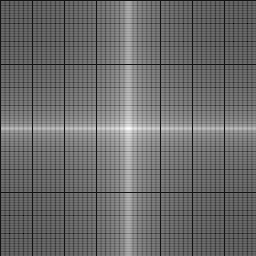
\includegraphics[angle=0,width=0.45\textwidth]{images/fft1}}\\
    \subfloat[Original]{\label{org_2}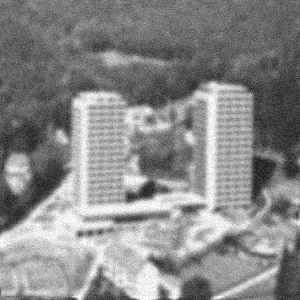
\includegraphics[angle=0,width=0.45\textwidth]{images/img2}}\hspace{1em}
    \subfloat[Fourier transform]{\label{ft_2}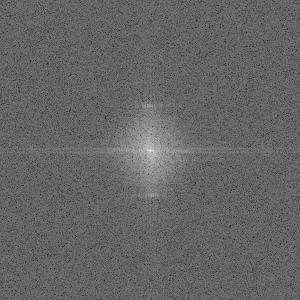
\includegraphics[angle=0,width=0.45\textwidth]{images/fft2}}
    \caption[]{Fourier transform of two pictures. On the left we have
    the original picture with its corresponding Fourier transform on the
    right.}
    \label{fourier_transforms}
\end{figure}

\begin{figure}[!h]
    \centering
    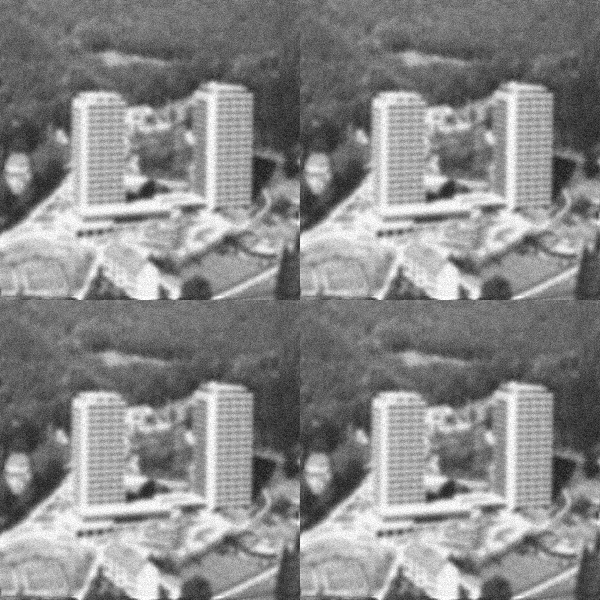
\includegraphics[angle=0,width=0.70\textwidth]{images/period}
    \caption[]{Periodicity in the noisy image. Notice that the pixel
    value are almost the same in the top of the image. When the images
    are put next to each other, it seem as there is no real boundary
    between them. This accounts for the missing vertical line in the
    Fourier transform in \textbf{fig. \ref{ft_2}}. When the images are
    put on top of each other, theres a clear line indicating where the
    image boundary is.}
    \label{period}
\end{figure}

\subsection*{Question 2.2}
We wish to find the Fourier transform $\hat{G}_{\sigma}(k)$ of the
gaussian distribution $G_{\sigma}(x)$.
\begin{align}
    \hat{G}_{\sigma}(k) & = \int_{-\infty}^{\infty}{\frac{1}{\sqrt{2\pi \sigma^{2}}}e^{-\frac{x^2}{2\sigma^2}}e^{-2\pi ikx}dx}\\
    & = \frac{1}{\sqrt{2\pi \sigma^{2}}}\int_{-\infty}^{\infty}{e^{-(\frac{1}{2\sigma^2}x^2 + 2\pi ikx)}dx}\\
    & = \frac{1}{\sqrt{2\pi
    \sigma^{2}}}\sqrt{\pi/\frac{1}{2\sigma^{2}}}e^{(2\pi ik)^2/\frac{4}{2\sigma^2}}\\
    & = e^{-2(\pi k\sigma)^2}
\end{align}
A lot things is going on. First, from (2) to (3), we have used that
\begin{equation}
    \int_{-\infty}^{\infty}e^{-(ax^2+bx+c)} = \sqrt{\pi/a}e^{b^2 - 4ac/4a}
\end{equation}
where $a = \frac{1}{2\sigma^2}$, $b = 2\pi ik$ and $c = 0$. From
(3) to (4) we rewrite some fractions. In (3) we have that
\begin{equation}
    \sqrt{\pi/\frac{1}{2\sigma^{2}}} =
    \sqrt{\pi\frac{2\sigma^2}{1}} = \sqrt{2\pi\sigma^2}
\end{equation}
which then eliminates the first term. Also, in the exponential function,
we have that
\begin{equation}
    (2\pi ik)^2 / \frac{4}{2\sigma^2} = \frac{-8\pi^{2}k^{2}\sigma^2}{4}
    = -2\pi^2 k^2\sigma^2 = -2(\pi k \sigma)^2
\end{equation}
where we notice the change in sign caused by $i^2 = -1$.

Just to recap, the Fourier transform of $G_{\sigma}(x)$ is
\begin{align}
    \hat{G}_{\sigma}(k) & = e^{-2(\pi k\sigma)^2}
\end{align}

We then define
\begin{align}
    h_1(x) & = G_{\sigma}(x)\cos(2\pi u_0x)\\
    h_2(x) & = G_{\sigma}(x)\sin(2\pi u_0x)\\
    h(x) & = h_1(x) + ih_2(x)
\end{align}
and we want to find the Fourier transform $\hat{h}(k)$ of $h(x)$.

We know $\hat{G}_{\sigma}(k)$ as well as the Fourier transforms of both
$\cos(2\pi u_0 x)$ and $\sin(2\pi u_0 x)$, see \citet[p.
557]{jahne-digital}. The convolution theorem says, that the convolution
of two functions in the Fourier domain means multiplication in the space
domain. Therefore, instead of multiplying the functions and then finding
the Fourier transform, we just convolve their Fourier transforms.
\begin{align}
    \hat{h}(x) & = \hat{G}_{\sigma}(k) \star \hat{h_1}(k) + i\hat{G}_{\sigma}(k) \star \hat{h_2}(k)\\
     & = \hat{G}_{\sigma}(k) \star (\hat{h_1}(k) + i\hat{h_2}(k))\\
     & = \hat{G}_{\sigma}(k) \star \left(\frac{\delta_{x - x_0} + \delta_{x + x_0}}{2} + i\frac{i\delta_{x - x_0} - \delta_{x + x_0}}{2}\right)\\
     & = \hat{G}_{\sigma}(k) \star \left(\frac{\delta_{x - x_0} + \delta_{x + x_0}}{2} - \frac{\delta_{x - x_0} - \delta_{x + x_0}}{2}\right)\\
     & = \hat{G}_{\sigma}(k) \star \delta_{x + x_0}\\
     & = \int_{-\infty}^{\infty}{e^{-2(\pi\sigma u_0)^2}\delta_{x + u_0}du_0}\\
     & = e^{-2(\pi\sigma u_0)^2}
\end{align}

The function $h(x)$ is defined on the form $r(cos(\theta) +
i\sin(\theta))$, where $r = G_{\sigma}(x)$, thus we have a complex
number based on the gaussian function. Therefore it is no surprise that
the Fourier transform yields the same result as the Fourier transform of
the gaussian function. The result is also a gaussian function of the
form $f(x) = e^{ax^2 + bx + x}$.

\subsection*{Question 2.3}
Given two continuous signals $f(x)$ and $g(x)$ we wish to find the
convolution $f \star g$. The two signals are shown in fig.
\ref{signals}.

\begin{figure}[!h]
    \centering
    \subfloat[$f(x)$]{\mbox{
    \begin{picture}(150,70)
        \put(60, 47){$A$}
        \put(105, 0){$1$}
        %\put(0, 45){\circle*{3}}

        {
        \color{red}
        \linethickness{1.6pt}
        \put(70, 50){\line(1, 0){35}}
        \put(0, 15){\line(1, 0){70}}
        \put(105, 15){\line(1, 0){31}}
        \put(70, 15){\line(0, 1){35}}
        \put(105, 15){\line(0, 1){35}}
        }

        \put(0, 15){\vector(1, 0){140}}
        \put(70, 15){\vector(0, 1){50}}

    \end{picture}}
    }\hspace{1em}
    \subfloat[$g(x)$]{\mbox{
    \begin{picture}(150,70)
        \put(25, 47){$B$}
        \put(105, 0){$1$}
        \put(30, 0){$-1$}
        %\put(0, 45){\circle*{3}}

        {
        \color{blue}
        \linethickness{1.6pt}
        \put(35, 50){\line(1, 0){70}}
        \put(0, 15){\line(1, 0){35}}
        \put(105, 15){\line(1, 0){31}}
        \put(35, 15){\line(0, 1){35}}
        \put(105, 15){\line(0, 1){35}}
        }

        \put(0, 15){\vector(1, 0){140}}
        \put(70, 15){\vector(0, 1){50}}

    \end{picture}}
    }
    \caption{Two signals}
    \label{signals}
\end{figure}

Convolution of two continuous signals is defined as
\begin{equation}
    (g \star f)(x) = \int_{-\infty}^{\infty}{f(\alpha)g(x - \alpha)d\alpha}
\end{equation}
where we have used that convolution is commutative. The signals are only
defined on certain intervals, thus we need to find these integration
limits to perform convolution. We also note that $A$ and $B$ only are
constants, thus we can replace them by $1$ and multiply later.

\begin{figure}[!h]
    \centering
    \subfloat[$(g \star f)(x)$]{\mbox{
    \begin{picture}(150,70)
        \put(-5, 47){$1$}
        \put(40, 65){$\alpha$}
        \put(75, 0){$x$}
        \put(105, 0){$1$}
        \put(30, 0){$-1$}
        %\put(0, 45){\circle*{3}}

        {
        \color{red}
        \linethickness{1.6pt}
        \put(75, 50){\line(1, 0){35}}
        \put(5, 15){\line(1, 0){70}}
        \put(110, 15){\line(1, 0){31}}
        %\put(70, 15){\line(0, 1){35}}
        \put(110, 15){\line(0, 1){35}}
        }

        {
        \color{blue}
        \put(35, 10){\line(0, 1){45}}
        \linethickness{1.6pt}
        \put(0, 50){\line(1, 0){70}}
        \put(-10, 15){\line(1, 0){10}}
        \put(75, 15){\line(1, 0){31}}
        \put(0, 15){\line(0, 1){35}}
        \put(70, 15){\line(0, 1){35}}
        }

        \put(0, 15){\vector(1, 0){140}}
        \put(70, 15){\vector(0, 1){50}}

    \end{picture}}
    }\hspace{1em}
    \subfloat[$(g \star f)(x)$]{\mbox{
    \begin{picture}(150,70)
        \put(60, 47){$1$}
        \put(145, 65){$\alpha$}
        \put(75, 0){$x$}
        \put(105, 0){$1$}
        \put(145, 0){$2$}
        \put(30, 0){$-1$}
        %\put(0, 45){\circle*{3}}

        {
        \color{red}
        \linethickness{1.6pt}
        \put(75, 50){\line(1, 0){35}}
        \put(5, 15){\line(1, 0){70}}
        \put(110, 15){\line(1, 0){31}}
        \put(75, 15){\line(0, 1){35}}
        \put(110, 15){\line(0, 1){35}}
        }

        {
        \color{blue}
        \put(140, 10){\line(0, 1){45}}
        \linethickness{1.6pt}
        \put(105, 50){\line(1, 0){70}}
        \put(-100, 15){\line(1, 0){10}}
        \put(175, 15){\line(1, 0){31}}
        \put(105, 15){\line(0, 1){35}}
        \put(175, 15){\line(0, 1){35}}
        }

        \put(0, 15){\vector(1, 0){140}}
        \put(70, 15){\vector(0, 1){50}}

    \end{picture}}
    }
    \caption{Convolution of two signals}
    \label{signals_outer}
\end{figure}
We mirror $g(x)$ and ``slide'' it over $f(x)$ and from fig.
\ref{signals_outer} we see that the outer limits of the integral are
$\alpha < -1$ and $\alpha \geq 2$, as the signals do not interfere with
each other. Thus we have
\begin{equation}
    \int_{-\infty}^{-1}{f(\alpha)g(x - \alpha)d\alpha} =
    \int_{2}^{\infty}{f(\alpha)g(x - \alpha)d\alpha} = 0
\end{equation}
We see that if we move $g(x)$ further than $-1$ the signals overlap. We
have a new limit $-1 \leq \alpha < 0$ and we use the convolution
integral:
\begin{equation}
    AB\int_{- 1}^{x}d\alpha = AB[\alpha]^{x}_{- 1} = AB(x + 1)
\end{equation}
Next, from 0 to 1, we can move $g(x)$ all the way across $f(x)$. We have
\begin{equation}
    AB\int_{0}^{1}d\alpha = AB[\alpha]^{1}_{0} = AB
\end{equation}
When $\alpha$ passes 1 the area of the intersection get linearly
smaller until 2, where the signal is zero for both. We integrate from
$x$ to 2:
\begin{equation}
    AB\int_{x}^{2}d\alpha = AB[\alpha]^{2}_{x} = AB(2-x)
\end{equation}
The final convolution of $f(x)$ and $g(x)$ is then defined as
\begin{equation}
    (g \star f)(x) =
    \left\{ \begin{array}{l l r}
        AB(x + 1) & \mbox{if} & -1 \leq x < 0\\
        AB & \mbox{if} & 0 \leq x < 1\\
        AB(2 - x) & \mbox{if} & 1 \leq x < 2\\
        0 & \mbox{otherwise} & \\
    \end{array}
    \right.
\end{equation}
and the signal is shown in fig. \ref{signals_final}.
\begin{figure}[!h]
    \centering
    \mbox{
    \begin{picture}(150,70)
        \put(45, 47){$AB$}
        \put(135, 0){$2$}
        \put(30, 0){$-1$}

        {
        \color{green}
        \linethickness{1.6pt}
        \put(70, 50){\line(1, 0){35}}
        \put(35, 15){\line(1, 1){35}}
        \put(105, 50){\line(1, -1){35}}
        \put(5, 15){\line(1, 0){30}}
        \put(140, 15){\line(1, 0){31}}
        }

        \put(0, 15){\vector(1, 0){175}}
        \put(70, 15){\vector(0, 1){50}}

    \end{picture}}
    \caption{Signal of $(f \star g)(x)$}
    \label{signals_final}
\end{figure}

\subsection*{Question 2.4}
We want to convolve the discrete function $h(x) =
[\frac{1}{3}~\frac{1}{3}~\frac{1}{3}]$ with itself 1, 2 and 3 times. The
original signal have been plotted in fig. \ref{org_plot}.

We define $h_1 = (h \star h)(x)$, $h_2 = (h \star h_1)(x)$ and $h_3 = (h
\star h_2)(x)$. The convolutions are solved trivially and we get the
signals
\begin{align}
    h_1 & =
    \left[\frac{1}{9}~\frac{2}{9}~\frac{3}{9}~\frac{2}{9}~\frac{1}{9}\right]\\
    h_2 & =
    \left[\frac{1}{27}~\frac{3}{27}~\frac{6}{27}~\frac{7}{27}~\frac{6}{27}~\frac{3}{27}~\frac{1}{27}\right]\\
    h_3 & =
    \left[\frac{1}{81}~\frac{4}{81}~\frac{10}{81}~\frac{16}{81}~\frac{19}{81}~\frac{16}{81}~\frac{10}{81}~\frac{4}{81}~\frac{1}{81}\right]
\end{align}
We note that the length of the signals increase with 2 for each
convolution. The convolutions are plotted in fig. \ref{1st} to
\ref{3rd}. For each convolution, we notice an increasing bell-shape
which indicate that we are approximating a gaussian function.  $h_2(x)$
and $h_3(x)$ have a lower peak value then $h_1(x)$ (and $h(x)$).

\begin{figure}[!h]
    \centering
    \subfloat[Original
    signal]{\label{org_plot}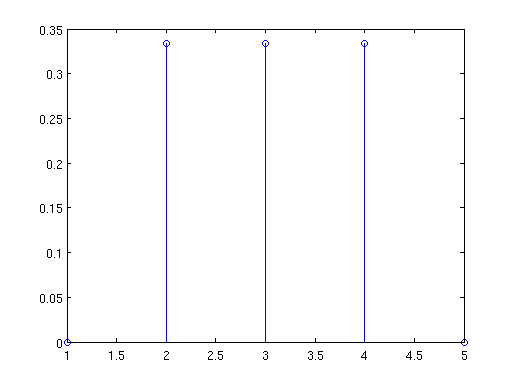
\includegraphics[angle=0,width=0.45\textwidth]{images/h_plot}}\hspace{1em}
    \subfloat[1$^{st}$
    convolution]{\label{1st}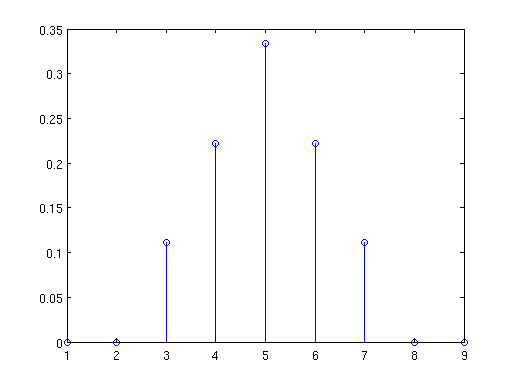
\includegraphics[angle=0,width=0.45\textwidth]{images/h_1st_plot}}\\
    \subfloat[2$^{nd}$
    convolution]{\label{2nd}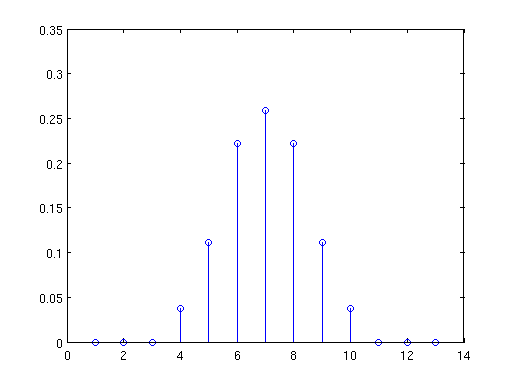
\includegraphics[angle=0,width=0.45\textwidth]{images/h_2nd_plot}}\hspace{1em}
    \subfloat[3$^{rd}$
    convolution]{\label{3rd}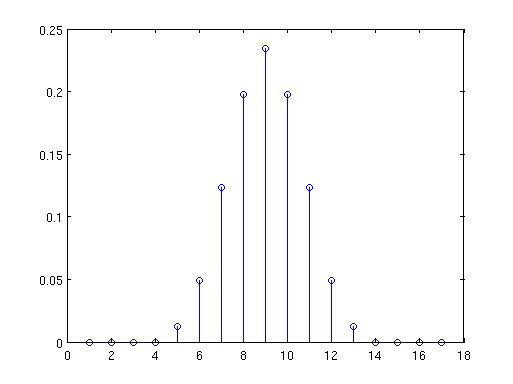
\includegraphics[angle=0,width=0.45\textwidth]{images/h_3rd_plot}}
    \caption[]{Consecutive convolution of the same function with itself.
    We approximate a gaussian function. Plots are made with MATLAB.}
    \label{sequence_scale}
\end{figure}

%%%%%%%%%%%%%%%%%%%%%%%%%%%%%%%%%%%%%%%%%%%%%%%%%%%%%%%%%%%%%%%%%%%%
% Formal stuff

\bibliographystyle{abbrvnat}
\bibliography{bibliography}
%\addcontentsline{toc}{chapter}{Litteratur}

\end{document}

% vim: set tw=72 spell spelllang=en:
